\documentclass[10pt,a4paper]{article}

\usepackage[top=11mm,bottom=9mm,left=12mm,right=12mm]{geometry}
\usepackage[T1]{fontenc}
\usepackage{tgheros}
\renewcommand{\familydefault}{\sfdefault}
\usepackage{microtype}
\usepackage{amsmath}

\usepackage[dvipsnames,svgnames,x11names]{xcolor}
\definecolor{bg}{HTML}{0E0E11}
\definecolor{cardbg}{HTML}{1F2937}
\definecolor{cyan}{HTML}{00D4FF}
\definecolor{gold}{HTML}{D4A574}
\definecolor{brightgold}{HTML}{FFD700}
\definecolor{crimson}{HTML}{E94560}
\definecolor{purple}{HTML}{8B5CF6}
\definecolor{emerald}{HTML}{10B981}
\definecolor{textmain}{HTML}{F0EDED}
\definecolor{textmuted}{HTML}{9CA3AF}
\definecolor{accentbar}{HTML}{00D4FF}

\usepackage{graphicx}
\graphicspath{{img/}}
\usepackage{tikz}
\usetikzlibrary{calc,positioning,backgrounds,fit}
\usepackage{multicol}
\usepackage{enumitem}
\usepackage{tabularx}
\usepackage{booktabs}
\usepackage{colortbl}
\usepackage{fontawesome5}
\usepackage{hyperref}
\hypersetup{colorlinks=true,urlcolor=cyan,linkcolor=cyan}
\usepackage{ragged2e}
\usepackage{setspace}

\pagecolor{bg}
\color{textmain}
\pagestyle{empty}

\setlength{\parindent}{0pt}
\setlength{\parskip}{1.5pt}
\setlength{\columnsep}{8mm}

\newcommand{\sectiontag}[1]{%
  \vspace{3pt}%
  {\scriptsize\color{gold}\MakeUppercase{#1}}\\[-2pt]%
}
\newcommand{\accentrule}{\textcolor{cyan}{\rule{\linewidth}{0.5pt}}}

\begin{document}

\begin{tikzpicture}[remember picture, overlay]
  \fill[accentbar] (current page.north west) rectangle ([yshift=-2pt]current page.north east);
\end{tikzpicture}

\vspace{-3mm}

% ── HEADER ──
\begin{minipage}[t]{0.60\linewidth}
  {\color{cyan}\Large$\diamondsuit$}\;\;{\LARGE\bfseries\color{textmain}VisionFlow}\\[1pt]
  {\normalsize\color{gold}Coordination Engineering for Federated Human--AI Intelligence}\\[2pt]
  {\scriptsize\color{textmuted}Open-source coordination harness. Diverse intelligence collaborates across trust boundaries at scale. Self-sovereign data. Formal reasoning. Cryptographic provenance. Human-in-the-loop governance.}
\end{minipage}%
\hfill
\begin{minipage}[t]{0.36\linewidth}
  \raggedleft
  \vspace{1pt}
  {\tiny
  \begin{tabular}{r@{\;}l}
    \color{textmuted}Maintainer & \bfseries Dr John O'Hare \\
    \color{textmuted}Org & \bfseries DreamLab AI \\
    \color{textmuted}Web & \href{https://www.visionflow.info}{visionflow.info} \\
    \color{textmuted}GitHub & \href{https://github.com/DreamLab-AI}{DreamLab-AI} \\
    \color{textmuted}Licence & VisionClaw: MPL 2.0 \\
    & Protocol stack: AGPL 3.0 \\
  \end{tabular}}
\end{minipage}

\vspace{2pt}
\accentrule
\vspace{1pt}

% ── STATS BAR — each stat is a minipage so number+label stay together ──
\begin{center}
\begin{minipage}[t]{0.13\linewidth}\centering
  {\large\bfseries\color{cyan}5}\\[-2pt]{\tiny\color{textmuted}Federated\\Substrates}
\end{minipage}\hfill
\begin{minipage}[t]{0.13\linewidth}\centering
  {\large\bfseries\color{cyan}92}\\[-2pt]{\tiny\color{textmuted}CUDA\\Kernels}
\end{minipage}\hfill
\begin{minipage}[t]{0.13\linewidth}\centering
  {\large\bfseries\color{cyan}185+}\\[-2pt]{\tiny\color{textmuted}MCP\\Tools}
\end{minipage}\hfill
\begin{minipage}[t]{0.13\linewidth}\centering
  {\large\bfseries\color{cyan}55\texttimes}\\[-2pt]{\tiny\color{textmuted}GPU\\Speedup}
\end{minipage}\hfill
\begin{minipage}[t]{0.13\linewidth}\centering
  {\large\bfseries\color{cyan}90+}\\[-2pt]{\tiny\color{textmuted}Agent\\Skills}
\end{minipage}\hfill
\begin{minipage}[t]{0.13\linewidth}\centering
  {\large\bfseries\color{cyan}6}\\[-2pt]{\tiny\color{textmuted}OSS\\Repos}
\end{minipage}
\end{center}

\vspace{1pt}
\accentrule

% ═══════════════════════════════════════════════
% MAIN CONTENT — TWO COLUMNS
% ═══════════════════════════════════════════════
\vspace{2pt}
\begin{multicols}{2}
\raggedright
\setstretch{0.92}

\sectiontag{Problem}
{\small\bfseries Hard problems share a common shape}\\[1pt]
{\scriptsize Climate modelling, drug discovery, creative production at scale. All require diverse intelligence collaborating across trust boundaries where centralised coordination breaks down.}

\vspace{1pt}
{\scriptsize\color{crimson}\bfseries 73\% of frontline AI adoption happens without management sign-off.} {\scriptsize\color{textmuted}Uncoordinated agents waste \textbf{60--80\% of tokens} on context rediscovery, duplicate reasoning, and contradictory outputs.}

\vspace{4pt}

\sectiontag{Why Token Vendors Should Care}
{\small\bfseries Coordination is the token multiplier}\\[1pt]

\begin{itemize}[leftmargin=8pt,itemsep=0pt,parsep=0pt,topsep=1pt,label={}]
  \item {\color{cyan}\textbullet} {\scriptsize\bfseries 3--5\texttimes{} effective throughput gain.} {\scriptsize\color{textmuted}Shared ontology eliminates re-derivation. Provenance eliminates re-validation. Governance prevents decision spin.}
  \item {\color{emerald}\textbullet} {\scriptsize\bfseries 10,000:1 problem-to-token ratio.} {\scriptsize\color{textmuted}\$2.6B drug compounds justify \$10K--100K in coordinated reasoning if one wrong conclusion is prevented.}
  \item {\color{gold}\textbullet} {\scriptsize\bfseries Break-even at 3 agents.} {\scriptsize\color{textmuted}Ontology, identity spine, governance are shared infra, not per-agent costs.}
  \item {\color{purple}\textbullet} {\scriptsize\bfseries Model-agnostic.} {\scriptsize\color{textmuted}Any LLM behind MCP tools. Multi-vendor consumption scales with problem complexity, not lock-in.}
\end{itemize}

\vspace{4pt}

\sectiontag{Architecture}
{\small\bfseries Five substrates, one cryptographic identity spine}\\[1pt]
{\scriptsize Every actor (human, agent, server) shares a single \texttt{did:nostr} secp256k1 keypair, verified at every layer.}

\vspace{3pt}

% ── Substrates as compact paragraphs, no tabularx ──
{\scriptsize
\textcolor{cyan}{\faProjectDiagram}\;\textbf{\color{cyan}VisionClaw} {\color{textmuted}| Knowledge Engineering}\\[-1pt]
{\color{textmuted}OWL\,2\,EL reasoning, 92 CUDA kernels, 55\texttimes{} GPU speedup, 3D graph, 17 MCP tools}

\vspace{2pt}
\textcolor{purple}{\faCogs}\;\textbf{\color{purple}Agentbox} {\color{textmuted}| Harness Engineering}\\[-1pt]
{\color{textmuted}90+ skills, 185+ MCP tools, governance relay, BIP-340 identity, Nix reproducible}

\vspace{2pt}
\textcolor{emerald}{\faLock}\;\textbf{\color{emerald}solid-pod-rs} {\color{textmuted}| Cryptographic Foundation}\\[-1pt]
{\color{textmuted}Rust Solid server, DID:Nostr + WAC + Web Ledgers, NIP-98 + OIDC + WebAuthn, HTTP\,402}

\vspace{2pt}
\textcolor{gold}{\faBalanceScale}\;\textbf{\color{gold}nostr-rust-forum} {\color{textmuted}| Governance UI}\\[-1pt]
{\color{textmuted}Judgment Broker, Agent Control Surface (kinds 31400--31405), Leptos WASM, passkey auth}

\vspace{2pt}
\textcolor{crimson}{\faGlobe}\;\textbf{\color{crimson}DreamLab Edge} {\color{textmuted}| Branded Deployment}\\[-1pt]
{\color{textmuted}React SPA + WASM forum, CF Workers edge, operator overlay, live at dreamlab-ai.com}
}

\vspace{4pt}

\sectiontag{Human-in-the-Loop Governance}
{\small\bfseries Judgment Broker}\\[1pt]
{\scriptsize Agent publishes control panel (kind\,31400) $\to$ forum renders to human $\to$ NIP-98 signed decision $\to$ VisionClaw gates knowledge mutations. Every decision is an immutable Nostr event. \textbf{90\% reduction in audit reconstruction cost.}}

\columnbreak

% ── RIGHT COLUMN ──
\sectiontag{Strategic Positioning: Wardley Map}
{\small\bfseries Every differentiator sits where no competitor can follow}\\[2pt]

\vspace{1pt}
\begin{center}
  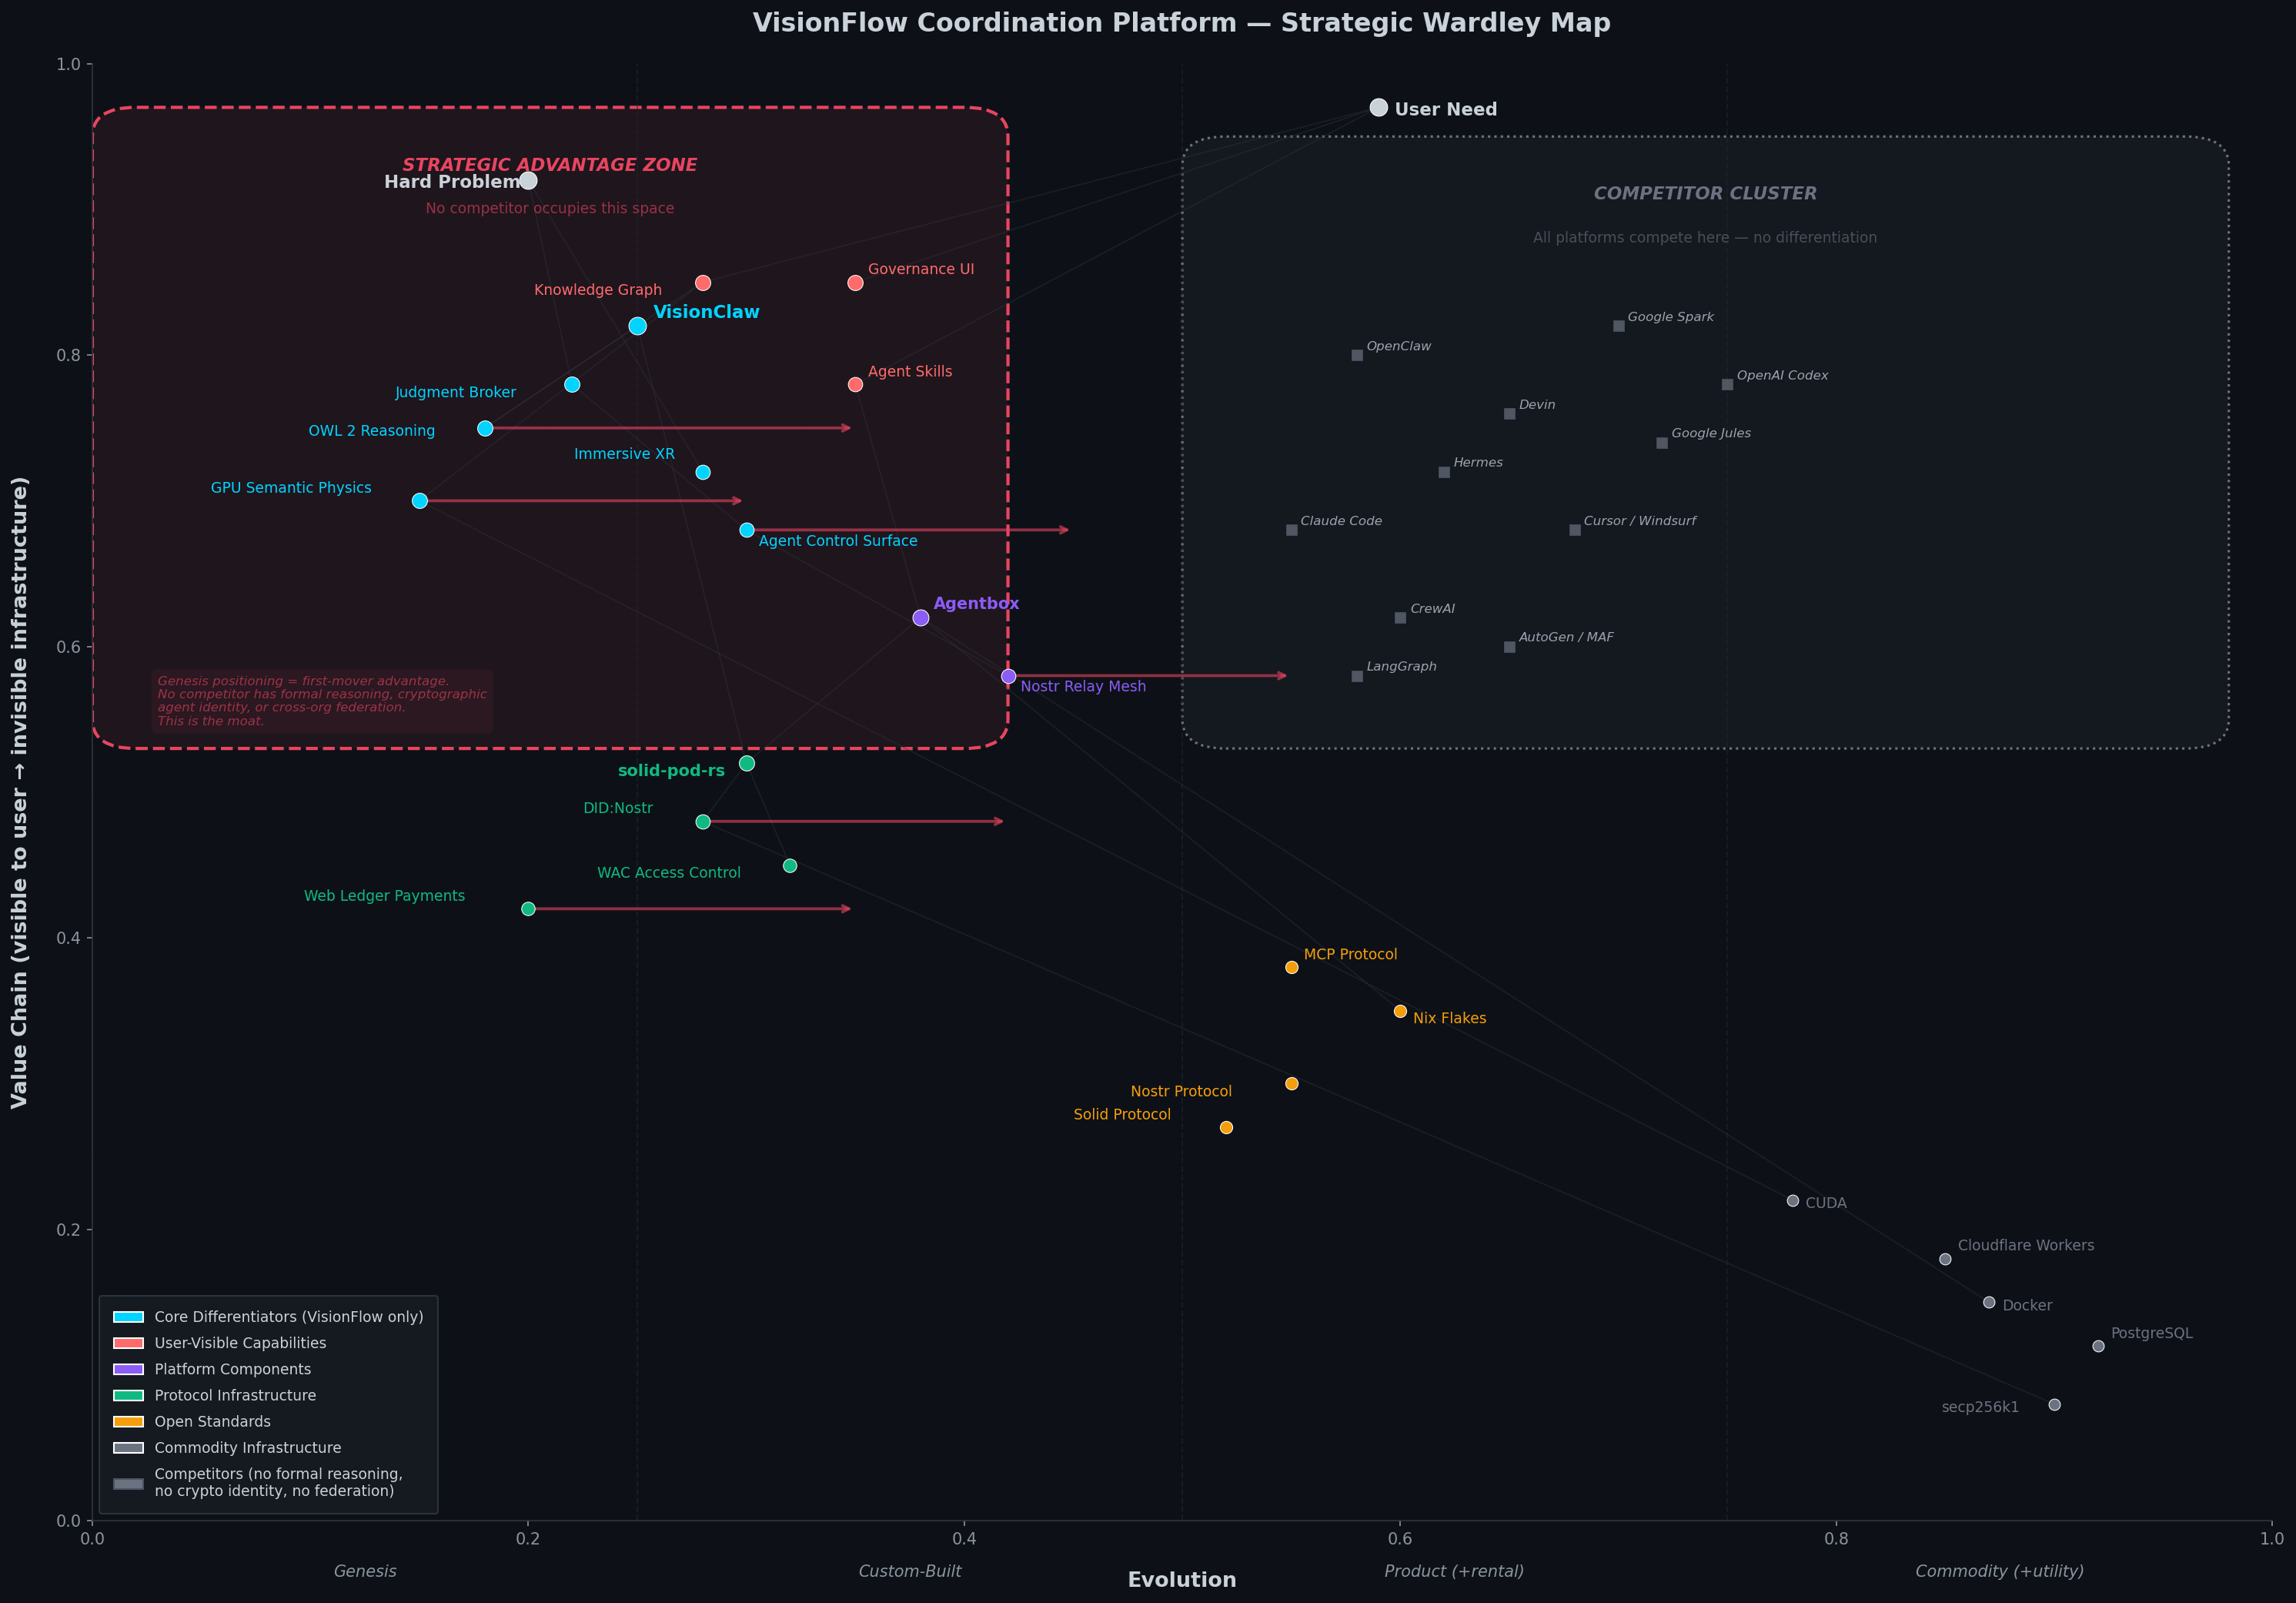
\includegraphics[width=\linewidth]{../assets/diagrams/wardley-map.png}
\end{center}

\vspace{1pt}
{\scriptsize\color{textmuted}%
VisionFlow's core differentiators ({\color{crimson}red zone, left}) occupy the genesis/custom-built quadrant: OWL\,2 formal reasoning, GPU semantic physics, Judgment Broker, cryptographic identity (DID:Nostr), immersive XR. No competitor has built here. All 11 competing platforms ({\color{textmuted}grey cluster, right}) sit in the commodity zone, interchangeable agent frameworks with no structural differentiation. The red dashed boundary marks the \textbf{strategic advantage zone}: capabilities that require deep protocol engineering. Cannot be replicated by wrapping an API.}

\vspace{4pt}

\sectiontag{Token Economics}
{\small\bfseries Tokenmaxing for hard problems is rational}\\[2pt]

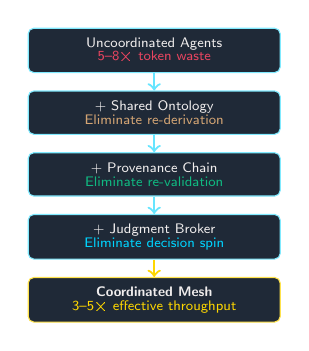
\begin{tikzpicture}[
  node distance=0.22cm,
  box/.style={draw=cyan!50,fill=cardbg,rounded corners=2pt,
              text=textmain,font=\tiny,align=center,
              minimum width=3.2cm,minimum height=0.55cm}
]
  \node[box] (a) {Uncoordinated Agents\\[-1pt]{\color{crimson}5--8\texttimes{} token waste}};
  \node[box,below=of a] (b) {+ Shared Ontology\\[-1pt]{\color{gold}Eliminate re-derivation}};
  \node[box,below=of b] (c) {+ Provenance Chain\\[-1pt]{\color{emerald}Eliminate re-validation}};
  \node[box,below=of c] (d) {+ Judgment Broker\\[-1pt]{\color{cyan}Eliminate decision spin}};
  \node[box,below=of d,draw=brightgold!70] (e) {\bfseries Coordinated Mesh\\[-1pt]{\color{brightgold}3--5\texttimes{} effective throughput}};
  \draw[->,cyan!60,thick] (a) -- (b);
  \draw[->,cyan!60,thick] (b) -- (c);
  \draw[->,cyan!60,thick] (c) -- (d);
  \draw[->,brightgold,thick] (d) -- (e);
\end{tikzpicture}

\vspace{3pt}

\sectiontag{Scaling}
{\scriptsize
\textcolor{emerald}{\faUser}\;\textbf{Single Operator} {\color{textmuted}| One API key, one container, minutes to deploy.}

\vspace{1pt}
\textcolor{gold}{\faUsers}\;\textbf{Team (50+)} {\color{textmuted}| Shared relay mesh, Judgment Broker oversight. Validated at scale.}

\vspace{1pt}
\textcolor{cyan}{\faNetworkWired}\;\textbf{Federated Enterprise} {\color{textmuted}| Sovereign nodes, trust via did:nostr. Horizontal scaling.}
}

\vspace{4pt}

\begin{center}

\begin{tikzpicture}
  \node[draw=cyan,fill=cardbg,rounded corners=3pt,
        text=textmain,font=\scriptsize,align=center,
        inner xsep=6pt,inner ysep=4pt] {
    \textbf{\color{brightgold}Open source. Model-agnostic. Federation-ready.}\\[1pt]
    {\tiny Every token produces auditable, governed, provenance-tracked reasoning.}\\[2pt]
    {\tiny\color{cyan}\href{https://github.com/DreamLab-AI}{github.com/DreamLab-AI}} \quad
    {\tiny\color{gold}\href{https://www.visionflow.info}{visionflow.info}} \quad
    {\tiny\color{emerald}\href{mailto:visionflow@thedreamlab.uk}{visionflow@thedreamlab.uk}}
  };
\end{tikzpicture}
\end{center}

\end{multicols}

\begin{tikzpicture}[remember picture, overlay]
  \fill[accentbar] (current page.south west) rectangle ([yshift=2pt]current page.south east);
\end{tikzpicture}

\end{document}
